% Options for packages loaded elsewhere
\PassOptionsToPackage{unicode}{hyperref}
\PassOptionsToPackage{hyphens}{url}
%
\documentclass[
]{article}
\usepackage{amsmath,amssymb}
\usepackage{iftex}
\ifPDFTeX
  \usepackage[T1]{fontenc}
  \usepackage[utf8]{inputenc}
  \usepackage{textcomp} % provide euro and other symbols
\else % if luatex or xetex
  \usepackage{unicode-math} % this also loads fontspec
  \defaultfontfeatures{Scale=MatchLowercase}
  \defaultfontfeatures[\rmfamily]{Ligatures=TeX,Scale=1}
\fi
\usepackage{lmodern}
\ifPDFTeX\else
  % xetex/luatex font selection
\fi
% Use upquote if available, for straight quotes in verbatim environments
\IfFileExists{upquote.sty}{\usepackage{upquote}}{}
\IfFileExists{microtype.sty}{% use microtype if available
  \usepackage[]{microtype}
  \UseMicrotypeSet[protrusion]{basicmath} % disable protrusion for tt fonts
}{}
\makeatletter
\@ifundefined{KOMAClassName}{% if non-KOMA class
  \IfFileExists{parskip.sty}{%
    \usepackage{parskip}
  }{% else
    \setlength{\parindent}{0pt}
    \setlength{\parskip}{6pt plus 2pt minus 1pt}}
}{% if KOMA class
  \KOMAoptions{parskip=half}}
\makeatother
\usepackage{xcolor}
\usepackage[margin=1in]{geometry}
\usepackage{color}
\usepackage{fancyvrb}
\newcommand{\VerbBar}{|}
\newcommand{\VERB}{\Verb[commandchars=\\\{\}]}
\DefineVerbatimEnvironment{Highlighting}{Verbatim}{commandchars=\\\{\}}
% Add ',fontsize=\small' for more characters per line
\usepackage{framed}
\definecolor{shadecolor}{RGB}{248,248,248}
\newenvironment{Shaded}{\begin{snugshade}}{\end{snugshade}}
\newcommand{\AlertTok}[1]{\textcolor[rgb]{0.94,0.16,0.16}{#1}}
\newcommand{\AnnotationTok}[1]{\textcolor[rgb]{0.56,0.35,0.01}{\textbf{\textit{#1}}}}
\newcommand{\AttributeTok}[1]{\textcolor[rgb]{0.13,0.29,0.53}{#1}}
\newcommand{\BaseNTok}[1]{\textcolor[rgb]{0.00,0.00,0.81}{#1}}
\newcommand{\BuiltInTok}[1]{#1}
\newcommand{\CharTok}[1]{\textcolor[rgb]{0.31,0.60,0.02}{#1}}
\newcommand{\CommentTok}[1]{\textcolor[rgb]{0.56,0.35,0.01}{\textit{#1}}}
\newcommand{\CommentVarTok}[1]{\textcolor[rgb]{0.56,0.35,0.01}{\textbf{\textit{#1}}}}
\newcommand{\ConstantTok}[1]{\textcolor[rgb]{0.56,0.35,0.01}{#1}}
\newcommand{\ControlFlowTok}[1]{\textcolor[rgb]{0.13,0.29,0.53}{\textbf{#1}}}
\newcommand{\DataTypeTok}[1]{\textcolor[rgb]{0.13,0.29,0.53}{#1}}
\newcommand{\DecValTok}[1]{\textcolor[rgb]{0.00,0.00,0.81}{#1}}
\newcommand{\DocumentationTok}[1]{\textcolor[rgb]{0.56,0.35,0.01}{\textbf{\textit{#1}}}}
\newcommand{\ErrorTok}[1]{\textcolor[rgb]{0.64,0.00,0.00}{\textbf{#1}}}
\newcommand{\ExtensionTok}[1]{#1}
\newcommand{\FloatTok}[1]{\textcolor[rgb]{0.00,0.00,0.81}{#1}}
\newcommand{\FunctionTok}[1]{\textcolor[rgb]{0.13,0.29,0.53}{\textbf{#1}}}
\newcommand{\ImportTok}[1]{#1}
\newcommand{\InformationTok}[1]{\textcolor[rgb]{0.56,0.35,0.01}{\textbf{\textit{#1}}}}
\newcommand{\KeywordTok}[1]{\textcolor[rgb]{0.13,0.29,0.53}{\textbf{#1}}}
\newcommand{\NormalTok}[1]{#1}
\newcommand{\OperatorTok}[1]{\textcolor[rgb]{0.81,0.36,0.00}{\textbf{#1}}}
\newcommand{\OtherTok}[1]{\textcolor[rgb]{0.56,0.35,0.01}{#1}}
\newcommand{\PreprocessorTok}[1]{\textcolor[rgb]{0.56,0.35,0.01}{\textit{#1}}}
\newcommand{\RegionMarkerTok}[1]{#1}
\newcommand{\SpecialCharTok}[1]{\textcolor[rgb]{0.81,0.36,0.00}{\textbf{#1}}}
\newcommand{\SpecialStringTok}[1]{\textcolor[rgb]{0.31,0.60,0.02}{#1}}
\newcommand{\StringTok}[1]{\textcolor[rgb]{0.31,0.60,0.02}{#1}}
\newcommand{\VariableTok}[1]{\textcolor[rgb]{0.00,0.00,0.00}{#1}}
\newcommand{\VerbatimStringTok}[1]{\textcolor[rgb]{0.31,0.60,0.02}{#1}}
\newcommand{\WarningTok}[1]{\textcolor[rgb]{0.56,0.35,0.01}{\textbf{\textit{#1}}}}
\usepackage{graphicx}
\makeatletter
\def\maxwidth{\ifdim\Gin@nat@width>\linewidth\linewidth\else\Gin@nat@width\fi}
\def\maxheight{\ifdim\Gin@nat@height>\textheight\textheight\else\Gin@nat@height\fi}
\makeatother
% Scale images if necessary, so that they will not overflow the page
% margins by default, and it is still possible to overwrite the defaults
% using explicit options in \includegraphics[width, height, ...]{}
\setkeys{Gin}{width=\maxwidth,height=\maxheight,keepaspectratio}
% Set default figure placement to htbp
\makeatletter
\def\fps@figure{htbp}
\makeatother
\setlength{\emergencystretch}{3em} % prevent overfull lines
\providecommand{\tightlist}{%
  \setlength{\itemsep}{0pt}\setlength{\parskip}{0pt}}
\setcounter{secnumdepth}{-\maxdimen} % remove section numbering
\usepackage{booktabs}
\usepackage{longtable}
\usepackage{array}
\usepackage{multirow}
\usepackage{wrapfig}
\usepackage{float}
\usepackage{colortbl}
\usepackage{pdflscape}
\usepackage{tabu}
\usepackage{threeparttable}
\usepackage{threeparttablex}
\usepackage[normalem]{ulem}
\usepackage{makecell}
\usepackage{xcolor}
\ifLuaTeX
  \usepackage{selnolig}  % disable illegal ligatures
\fi
\IfFileExists{bookmark.sty}{\usepackage{bookmark}}{\usepackage{hyperref}}
\IfFileExists{xurl.sty}{\usepackage{xurl}}{} % add URL line breaks if available
\urlstyle{same}
\hypersetup{
  hidelinks,
  pdfcreator={LaTeX via pandoc}}

\author{}
\date{\vspace{-2.5em}}

\begin{document}

\begin{Shaded}
\begin{Highlighting}[]
\CommentTok{\# Chargement des packages}
\FunctionTok{library}\NormalTok{(stringi)}
\FunctionTok{library}\NormalTok{(dplyr)}
\end{Highlighting}
\end{Shaded}

\begin{verbatim}
## 
## Attachement du package : 'dplyr'
\end{verbatim}

\begin{verbatim}
## Les objets suivants sont masqués depuis 'package:stats':
## 
##     filter, lag
\end{verbatim}

\begin{verbatim}
## Les objets suivants sont masqués depuis 'package:base':
## 
##     intersect, setdiff, setequal, union
\end{verbatim}

\begin{Shaded}
\begin{Highlighting}[]
\FunctionTok{library}\NormalTok{(knitr)}
\end{Highlighting}
\end{Shaded}

\begin{verbatim}
## Warning: le package 'knitr' a été compilé avec la version R 4.3.3
\end{verbatim}

\begin{Shaded}
\begin{Highlighting}[]
\FunctionTok{library}\NormalTok{(kableExtra)}
\end{Highlighting}
\end{Shaded}

\begin{verbatim}
## Warning: le package 'kableExtra' a été compilé avec la version R 4.3.3
\end{verbatim}

\begin{verbatim}
## 
## Attachement du package : 'kableExtra'
\end{verbatim}

\begin{verbatim}
## L'objet suivant est masqué depuis 'package:dplyr':
## 
##     group_rows
\end{verbatim}

\begin{Shaded}
\begin{Highlighting}[]
\FunctionTok{library}\NormalTok{(tidyr)}
\FunctionTok{library}\NormalTok{(tidyverse)}
\end{Highlighting}
\end{Shaded}

\begin{verbatim}
## Warning: le package 'ggplot2' a été compilé avec la version R 4.3.3
\end{verbatim}

\begin{verbatim}
## Warning: le package 'tibble' a été compilé avec la version R 4.3.3
\end{verbatim}

\begin{verbatim}
## -- Attaching core tidyverse packages ------------------------ tidyverse 2.0.0 --
## v forcats   1.0.0     v readr     2.1.4
## v ggplot2   3.5.1     v stringr   1.5.0
## v lubridate 1.9.3     v tibble    3.2.1
## v purrr     1.0.1
\end{verbatim}

\begin{verbatim}
## -- Conflicts ------------------------------------------ tidyverse_conflicts() --
## x dplyr::filter()          masks stats::filter()
## x kableExtra::group_rows() masks dplyr::group_rows()
## x dplyr::lag()             masks stats::lag()
## i Use the ]8;;http://conflicted.r-lib.org/conflicted package]8;; to force all conflicts to become errors
\end{verbatim}

\begin{Shaded}
\begin{Highlighting}[]
\FunctionTok{library}\NormalTok{(summarytools)}
\end{Highlighting}
\end{Shaded}

\begin{verbatim}
## Warning: le package 'summarytools' a été compilé avec la version R 4.3.3
\end{verbatim}

\begin{verbatim}
## 
## Attachement du package : 'summarytools'
## 
## L'objet suivant est masqué depuis 'package:tibble':
## 
##     view
\end{verbatim}

\begin{Shaded}
\begin{Highlighting}[]
\FunctionTok{library}\NormalTok{(gridExtra)}
\end{Highlighting}
\end{Shaded}

\begin{verbatim}
## 
## Attachement du package : 'gridExtra'
## 
## L'objet suivant est masqué depuis 'package:dplyr':
## 
##     combine
\end{verbatim}

\begin{Shaded}
\begin{Highlighting}[]
\FunctionTok{library}\NormalTok{(purrr)}
\FunctionTok{library}\NormalTok{(skimr)}
\end{Highlighting}
\end{Shaded}

\begin{verbatim}
## Warning: le package 'skimr' a été compilé avec la version R 4.3.3
\end{verbatim}

\begin{Shaded}
\begin{Highlighting}[]
\FunctionTok{library}\NormalTok{(spdep)}
\end{Highlighting}
\end{Shaded}

\begin{verbatim}
## Warning: le package 'spdep' a été compilé avec la version R 4.3.3
\end{verbatim}

\begin{verbatim}
## Le chargement a nécessité le package : spData
\end{verbatim}

\begin{verbatim}
## Warning: le package 'spData' a été compilé avec la version R 4.3.3
\end{verbatim}

\begin{verbatim}
## To access larger datasets in this package, install the spDataLarge
## package with: `install.packages('spDataLarge',
## repos='https://nowosad.github.io/drat/', type='source')`
## Le chargement a nécessité le package : sf
## Linking to GEOS 3.11.2, GDAL 3.6.2, PROJ 9.2.0; sf_use_s2() is TRUE
\end{verbatim}

\begin{Shaded}
\begin{Highlighting}[]
\FunctionTok{library}\NormalTok{(geosphere)}
\end{Highlighting}
\end{Shaded}

\begin{verbatim}
## Warning: le package 'geosphere' a été compilé avec la version R 4.3.3
\end{verbatim}

\hypertarget{analyse-descriptive}{%
\section{Analyse descriptive}\label{analyse-descriptive}}

\hypertarget{description-de-la-population}{%
\subsection{Description de la
population}\label{description-de-la-population}}

\hypertarget{pyramide-des-ages}{%
\subsubsection{Pyramide des ages}\label{pyramide-des-ages}}

Notre population d'étude est une population assez homogène en matière
d'âge. Cependant plus on dépasse les 75 ans et moins on rencontre de
personnes. D'autres part notre popuplation est fortement masculine avec
une forte proportion des hommes quelle que soit la tranche d'âge à
l'exception des tranches du troisième âge.

\begin{figure}

{\centering 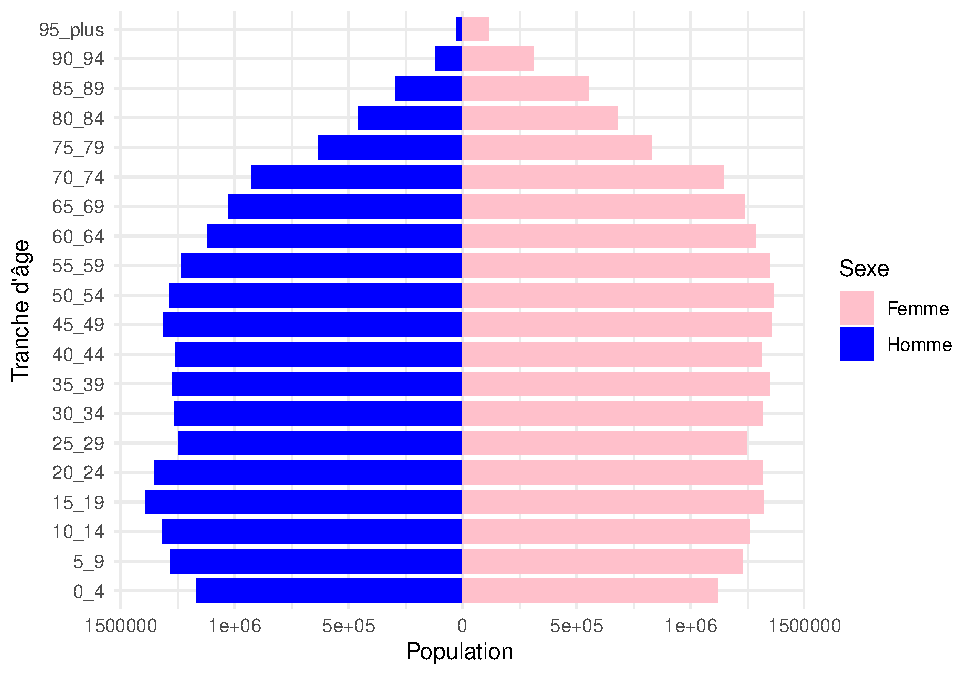
\includegraphics{4_Analyse_Descriptive_files/figure-latex/unnamed-chunk-3-1} 

}

\caption{Pyramide des âges}\label{fig:unnamed-chunk-3}
\end{figure}

\hypertarget{taux-de-natalituxe9-et-taux-de-mortalituxe9}{%
\subsubsection{Taux de natalité et taux de
mortalité}\label{taux-de-natalituxe9-et-taux-de-mortalituxe9}}

Dans les commmunes étudiées, le taux de natalité et de mortalité sont un
peu élevées avec la plupart des taux variant entre 5 et 15 pour 1000 en
ce qui concerne la natalité et 0 et 20 pour 1000 pour la mortalité. On
remarque une corrélation négative entre ces deux taux. Néanmoins cette
corrélation n'a à priori aucun sens. Par ailleurs, l'observation des
distributions permet de constater que la natalité est de façon générale
élevée par rapport à la mortalité dans les communes étudiées.

\begin{figure}

{\centering 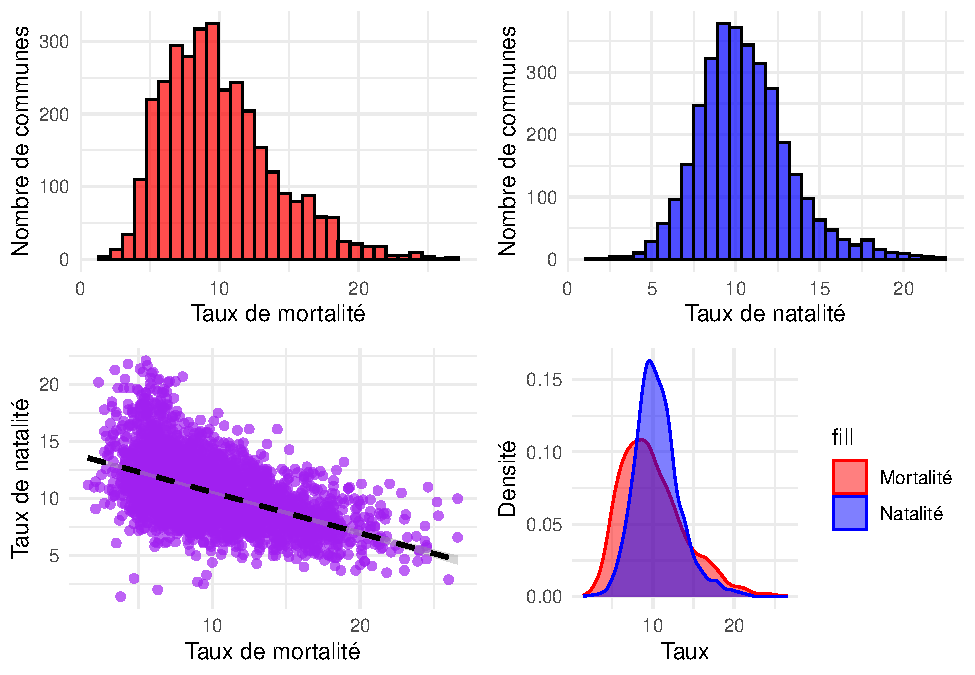
\includegraphics{4_Analyse_Descriptive_files/figure-latex/unnamed-chunk-4-1} 

}

\caption{Taux de Natalité et Taux de Mortalité}\label{fig:unnamed-chunk-4}
\end{figure}

En vue de mieux voir peut être l'effet de la mortalité sur la natalité,
nous allons nous intéresser alors à une analyse de la corrélation entre
les deux taux par groupe d'age. Nous avons considérer les groupes d'âge
suivants : 0-24, 25-44, 45-60, 60 et plus en fonction des variables
disponibles et ausi à partir de l'information sur l'âge des femmes en
âge de procréer qui est de l'ordre de 25-45 et des personnes âgées dont
l'âge est de plus 60 ans. Ne disposant pas du taux de mortalité dans
chaque groupe, alors nous avons dans notre analyse opté plutôt pour le
pourcentage des femmes de chaque groupe en partant du principe que la
natalité est très souvent liée aux femmes et du fait que nous pouvons
analyser une diminution du pourcentage comme étant dû à une mortalité.
Ainsi sur la base de cette nouvelle hypothèse, voici nos nouveaux
résultats.

\begin{figure}

{\centering 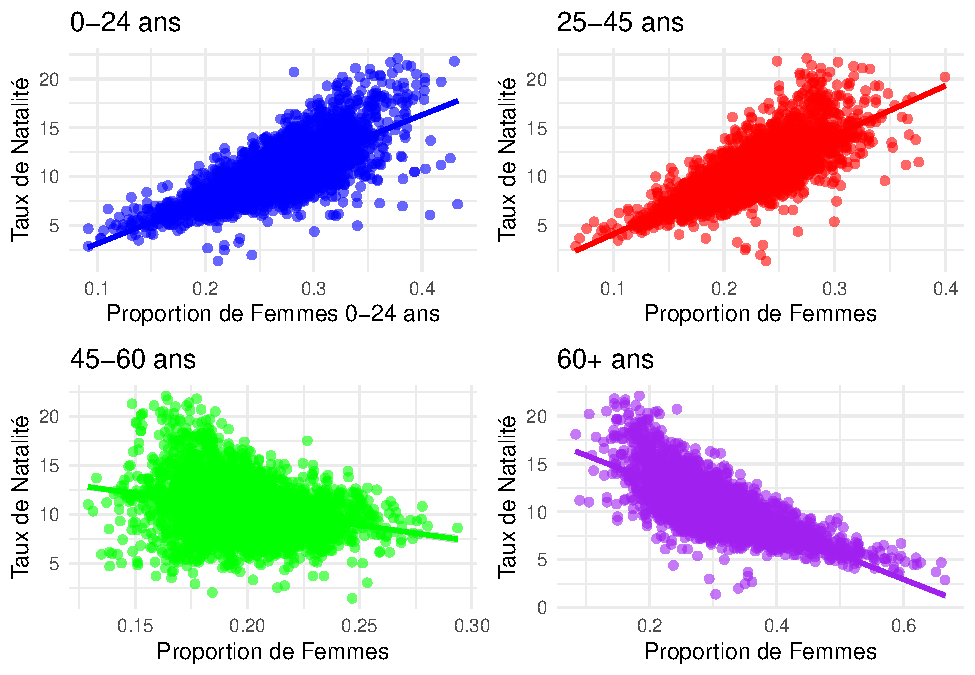
\includegraphics{4_Analyse_Descriptive_files/figure-latex/unnamed-chunk-5-1} 

}

\caption{Taux de Natalité et Pourcentage des femmes dans chaque groupe}\label{fig:unnamed-chunk-5}
\end{figure}

Les résultats nous montrent un lien croissant pour les tranches d'âge
0-24 et 25-45 ans montrant ainsi que dans ces tranches d'âge si le
pourcentage des femmes diminuent (quer l'on pourrait assimiler à une
mort des femmes) alors le taux de natalité diminue. Par ailleurs ceux de
la tranche 45-60 semble n'avoir aucun lien sur le taux de natalité.
Enfin il a été constaté un lien négatif pour la tranche d'âge 60 ans et
plus.

\hypertarget{taux-et-nombre-de-visites}{%
\subsection{Taux et nombre de visites}\label{taux-et-nombre-de-visites}}

(Insérer les cartes à ce niveau : Richard doit refaire les cartes et les
insérer)

L'analyse des statistiques descriptives sur le nombre de visites
annuelles de médecin généraliste entre 2018 et 2022 révèle une
distribution fortement asymétrique à droite, avec une grande dispersion
des données. La moyenne de 19130 visites, nettement supérieure à la
médiane de 9127, indique la présence de valeurs extrêmes tirant la
distribution vers le haut. Cette asymétrie est confirmée par l'écart
considérable entre le minimum de 1037 et le maximum de 765833 visites
par an.

\begin{figure}

{\centering 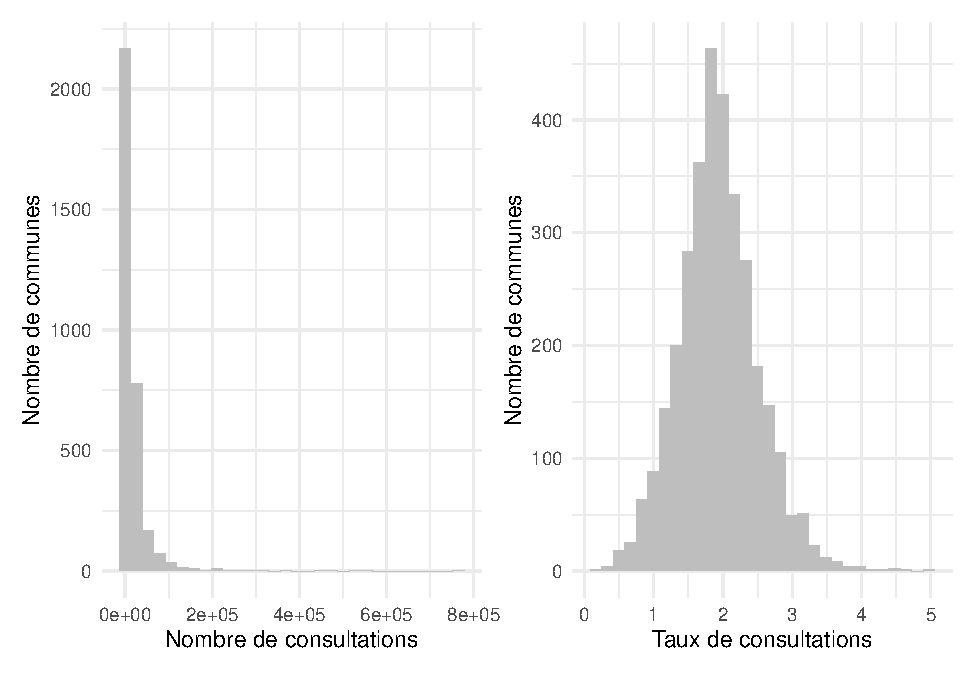
\includegraphics{4_Analyse_Descriptive_files/figure-latex/unnamed-chunk-6-1} 

}

\caption{Distributiion du nombre et du taux de visites}\label{fig:unnamed-chunk-6}
\end{figure}

La moitié des médecins généralistes effectuent entre 5993 et 17290
consultations annuellement, ce qui suggère une variabilité importante
dans la charge de travail. La médiane de 9127 consultations par an,
équivalant à environ 25 consultations par jour ouvrable, semble plus
représentative de l'activité typique d'un médecin généraliste que la
moyenne influencée par les valeurs extrêmes. Ces statistiques mettent en
lumière la diversité des pratiques et des charges de travail parmi les
médecins généralistes, avec potentiellement quelques cas atypiques
présentant un volume de consultations exceptionnellement élevé.

Le nombre de visites pouvant potentiellement être influencé par la
taille de la commune et donc par sa population, nous avons éliminer cet
effet en calculant le taux de consultations qui n'est autre que le
nombre de consultations moyennes par personnes.

\begin{table}[H]
\centering
\caption{\label{tab:unnamed-chunk-7}Résumé statistique du nombre de visites}
\centering
\begin{tabular}[t]{rrrrrr}
\toprule
Min. & 1st Qu. & Median & Mean & 3rd Qu. & Max.\\
\midrule
\cellcolor{gray!10}{1037} & \cellcolor{gray!10}{5993} & \cellcolor{gray!10}{9127} & \cellcolor{gray!10}{19129.63} & \cellcolor{gray!10}{17290} & \cellcolor{gray!10}{765833}\\
\bottomrule
\end{tabular}
\end{table}

\hypertarget{taux-de-visites-et-quelques-variables-duxe9mographiques-et-socio-uxe9conomiques}{%
\subsection{Taux de visites et quelques variables démographiques et
socio-économiques}\label{taux-de-visites-et-quelques-variables-duxe9mographiques-et-socio-uxe9conomiques}}

Nous allons ici, voir s'il y a un lien à priori entre le taux de visites
et certaines de nos variables explicatives. Ainsi, nous avons d'abord
réalisé une analyse descriptive bivariée puis nous avons calculé la
corrélation de Pearson pour évaluer le lien linéaire entre le taux de
consulation et des variables telles que la population totale, la part
des personnes agées (75 ans et plus), la part de quelques CSP (ouvriers
et retraités).

\hypertarget{taux-de-visites-et-population-totale}{%
\subsubsection{Taux de visites et population
totale}\label{taux-de-visites-et-population-totale}}

En divisant les communes en trois groupes égaux (ou presque égaux) en
fonction de la population totale, il ressort un lien clair entre la
taille des communes françaises et le taux de visites médicales, mettant
en évidence une tendance où les grandes communes (\textgreater{} 8974
habitants) affichent un taux moyen de visites supérieur (1,526810) par
rapport aux communes moyennes (1,456356) et petites (1,383861). Cette
observation suggère que l'accès facilité aux infrastructures médicales
dans les zones urbaines contribue à une utilisation accrue des services
de santé. En revanche, les petites communes, probablement plus isolées
et moins dotées en praticiens, semblent rencontrer des barrières
structurelles limitant la fréquence des visites.

\begin{table}[H]
\centering
\caption{\label{tab:unnamed-chunk-8}Taux de visites selon la taille de la commune}
\centering
\begin{tabular}[t]{lr}
\toprule
taille\_commune & Taux de consulations\\
\midrule
\cellcolor{gray!10}{Grande (> 8974)} & \cellcolor{gray!10}{1.526810}\\
Moyenne (4849 - 8974) & 1.456356\\
\cellcolor{gray!10}{Petite (<= 4848)} & \cellcolor{gray!10}{1.383861}\\
\bottomrule
\end{tabular}
\end{table}

\hypertarget{taux-de-visites-et-population-uxe2guxe9e}{%
\subsubsection{Taux de visites et population
âgée}\label{taux-de-visites-et-population-uxe2guxe9e}}

L'analyse met en évidence que les communes françaises avec une
population âgée significative (population âgée de 75 ans et plus est
supérieure à la médiane soit plus de 670 habitants âgés de 75 ans et
plus) présentent un taux moyen de visistes inférieur (1,410213) comparé
aux communes où la population âgée est moindre (1,501111). Cette
observation peut refléter des défis spécifiques aux populations plus
âgées, tels que des obstacles physiques ou logistiques pour accéder aux
soins médicaux, ou encore une moindre propension à consulter
régulièrement en raison d'habitudes ou de conditions de santé
chroniques. Ces résultats soulignent un paradoxe apparent, car les
besoins en soins médicaux des personnes âgées sont en général plus
importants, ce qui pourrait indiquer une inadéquation entre l'offre
médicale et les besoins spécifiques de cette tranche d'âge. Cela met en
lumière un enjeu crucial pour les politiques de santé visant à améliorer
l'accès et l'utilisation des services médicaux pour les populations
vieillissantes.

\begin{table}[H]
\centering
\caption{\label{tab:unnamed-chunk-9}Taux de visites selon la population âgée}
\centering
\begin{tabular}[t]{lr}
\toprule
population\_agee\_importante & consultations\_moyennes\\
\midrule
\cellcolor{gray!10}{Non (<= 670)} & \cellcolor{gray!10}{1.501111}\\
Oui (> 670) & 1.410213\\
\bottomrule
\end{tabular}
\end{table}

\hypertarget{taux-de-visites-et-csp}{%
\subsubsection{Taux de visites et CSP}\label{taux-de-visites-et-csp}}

Aucune catégorie ne semble montrer une relation linéaire évidente avec
le taux de visites. Par ailleurs, pour toutes les catégories
socio-professionnelles, la majorité des communes se situent dans une
plage de proportions faibles, ce qui limite la variabilité observable
dans les relations. Une analyse statistique supplémentaire, comme le
calcul de corrélations, serait nécessaire pour confirmer ou infirmer les
relations observées visuellement.

\begin{figure}

{\centering 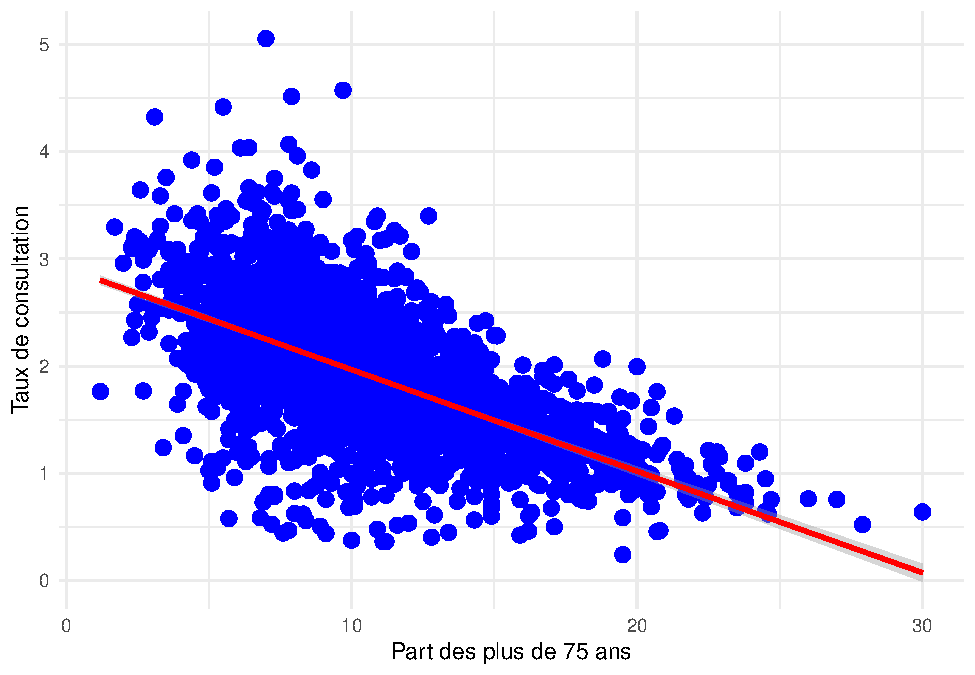
\includegraphics{4_Analyse_Descriptive_files/figure-latex/unnamed-chunk-10-1} 

}

\caption{Relations entre le taux de visites et certaines catégories socioprofessionnelles (variables standarisées)}\label{fig:unnamed-chunk-10}
\end{figure}

\hypertarget{trouver-un-titre-pour-cette-section-et-analyser-alex}{%
\subsubsection{(Trouver un titre pour cette section et analyser :
Alex)}\label{trouver-un-titre-pour-cette-section-et-analyser-alex}}

\begin{figure}

{\centering 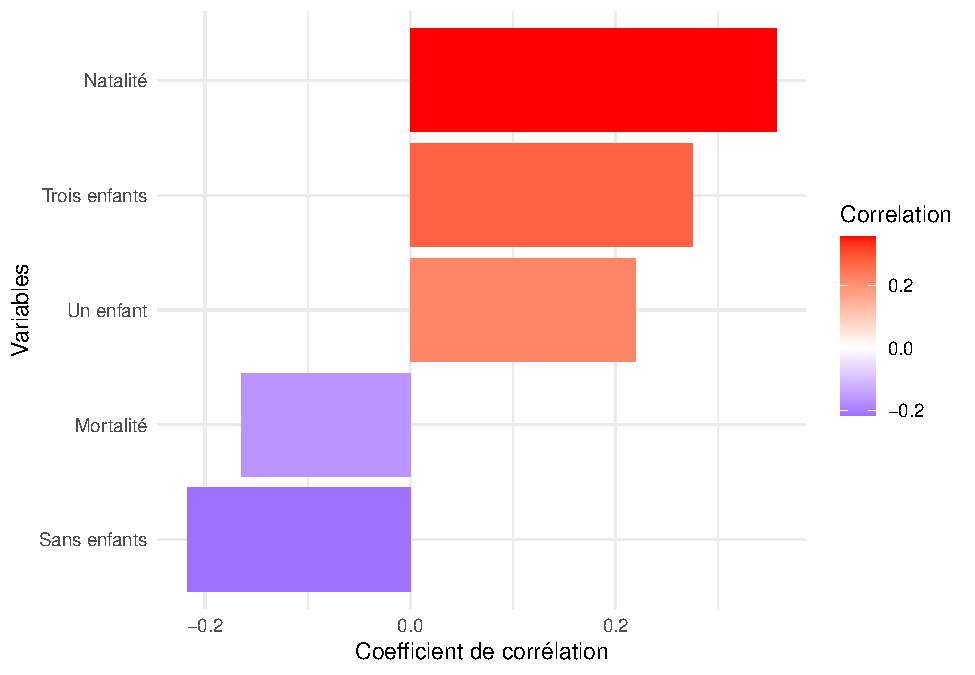
\includegraphics{4_Analyse_Descriptive_files/figure-latex/unnamed-chunk-11-1} 

}

\caption{Corrélations entre le nombre de visite et quelques variables}\label{fig:unnamed-chunk-11}
\end{figure}

\hypertarget{analyse-spatiale}{%
\subsection{Analyse spatiale}\label{analyse-spatiale}}

Après une analyse de nos données en ne tenant pas compte de l'effet
spatial, nous allons à présent poursuivre avec une analyse qui tient
compte de celui-ci. Nous allons ici faire une analyse basée sur le
diagramme de Moran. Ainsi d'après les explications données au niveau de
la partie méthodologie, nous aurons les 4 quadrants suivants.

\begin{itemize}
\tightlist
\item
  \textbf{Quadrant 1 (haut à droite)} : Les zones avec un taux de
  consultations plus élevé que la moyenne, entourées de zones présentant
  également un taux de consultations élevé (autocorrélation spatiale
  positive, structure \textbf{high-high}).
\item
  \textbf{Quadrant 3 (bas à gauche)} : Les zones avec un taux de
  consultations plus faible que la moyenne, entourées de zones
  présentant un taux de consultations également faible (autocorrélation
  spatiale positive, structure \textbf{low-low}).
\item
  \textbf{Quadrant 2 (bas à droite)} : Les zones avec un taux de
  consultations plus élevé que la moyenne, mais entourées de zones
  présentant un taux de consultations plus faible (autocorrélation
  spatiale négative, structure \textbf{high-low}).
\item
  \textbf{Quadrant 4 (haut à gauche)} : Les zones avec un taux de
  consultations plus faible que la moyenne, mais entourées de zones avec
  un taux de consultations plus élevé (autocorrélation spatiale
  négative, structure \textbf{low-high}).
\end{itemize}

Vu le nombre de nos communes, la mise sur le graphique des noms de
toutes les communes allait être compliquée. Pour cela, nous avons choisi
au hasard 4 communes par cadrant. Ainsi, Ce diagramme de Moran illustre
la corrélation spatiale des taux de consultation par commune et ceux des
communes voisines. La tendance générale, représentée par la droite de
régression rouge, montre une relation positive entre ces taux,
confirmant ainsi une autocorrélation spatiale. Autrement dit, les
communes ayant un taux élevé de consultations ont tendance à être
entourées par d'autres communes avec un taux similaire, et inversement.

Dans le quadrant HH (Haut-Haut), représenté en rouge, on retrouve des
communes comme Saint-Saulve, Le Bouscat et Bruay-la-Buissière. Celles-ci
affichent un taux de consultations élevé et sont entourées par des
communes présentant également des taux élevés. Cela indique une
concentration géographique des consultations médicales, qui peut
s'expliquer par une offre de soins plus développée ou une demande locale
particulièrement forte.

Le quadrant HL (Haut-Bas), en violet, comprend des communes comme
Saint-Jacques-de-la-Lande et Le Portel. Ces communes ont un taux élevé
de consultations, mais sont entourées de communes où les taux sont plus
faibles. Ce contraste peut suggérer que ces villes disposent d'une offre
de soins plus attractive que leurs voisines, attirant ainsi des patients
des alentours.

À l'inverse, dans le quadrant LH (Bas-Haut), en vert, on trouve des
communes comme Aix-en-Provence, Ribécourt-Dreslincourt et L'Isle-Adam.
Ces communes affichent un faible taux de consultations, tandis que leurs
voisines présentent des taux plus élevés. Ce phénomène peut s'expliquer
par le fait que les habitants de ces villes se rendent dans les communes
avoisinantes pour leurs consultations, soit en raison d'un manque
d'infrastructures médicales locales, soit par préférence pour des
services situés ailleurs.

Enfin, le quadrant LL (Bas-Bas), en orange, inclut des communes comme
Saint-Jean-le-Blanc, Romorantin-Lanthenay et Le Breuil. Ces villes ont
un faible taux de consultations et sont entourées de communes où les
taux sont également bas. Cela peut indiquer une accessibilité réduite
aux soins de santé, une moindre densité médicale, ou encore une faible
demande locale pour des consultations.

En résumé, cette analyse met en évidence des disparités territoriales
dans la répartition des consultations médicales. Certaines communes
concentrent les services et attirent les patients des alentours, tandis
que d'autres souffrent d'un accès limité aux soins, renforçant ainsi les
inégalités spatiales en matière de santé.

\begin{figure}

{\centering 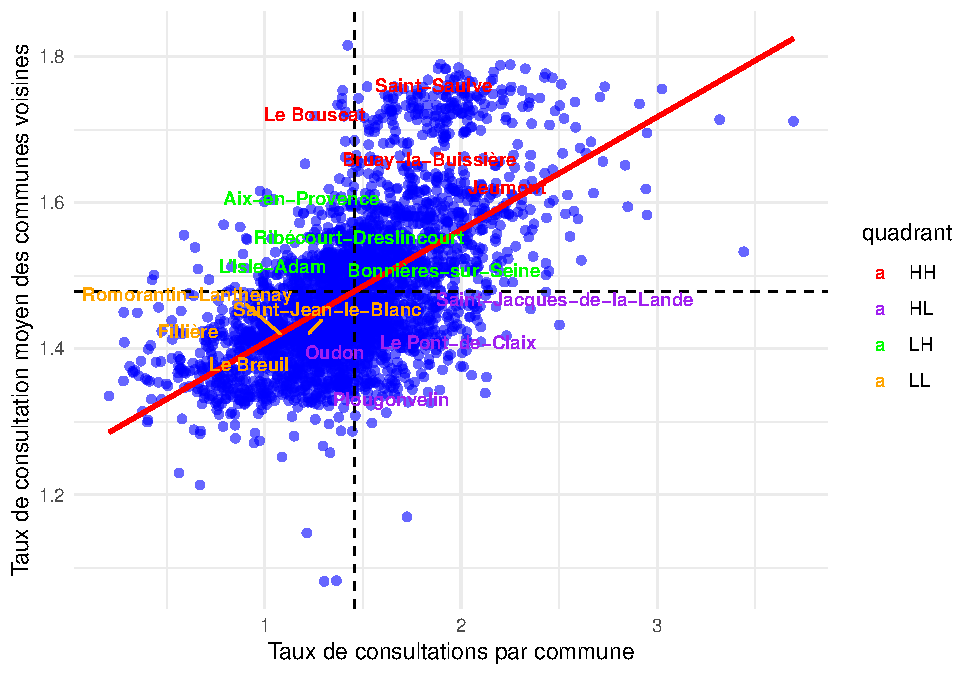
\includegraphics{4_Analyse_Descriptive_files/figure-latex/unnamed-chunk-19-1} 

}

\caption{Moran Plot avec visibilités de quelques communes}\label{fig:unnamed-chunk-19}
\end{figure}

\hypertarget{autocoruxe9lation-locale}{%
\subsubsection{Autocorélation locale}\label{autocoruxe9lation-locale}}

En se basant sur l'analyse par cluster fourni pour le LISA (local
Indicator or Spatial Association), nous pouvons remarquer que le cluster
HH est celui regroupant le plus de communes suivi du cluster LH. Ceci
dit une grande partie des communes ont des taux élevées et entourées par
des communes avec des taux élevés ou encore des taux bas et entourées
par des communes ayant des taux élevés.

\begin{figure}

{\centering 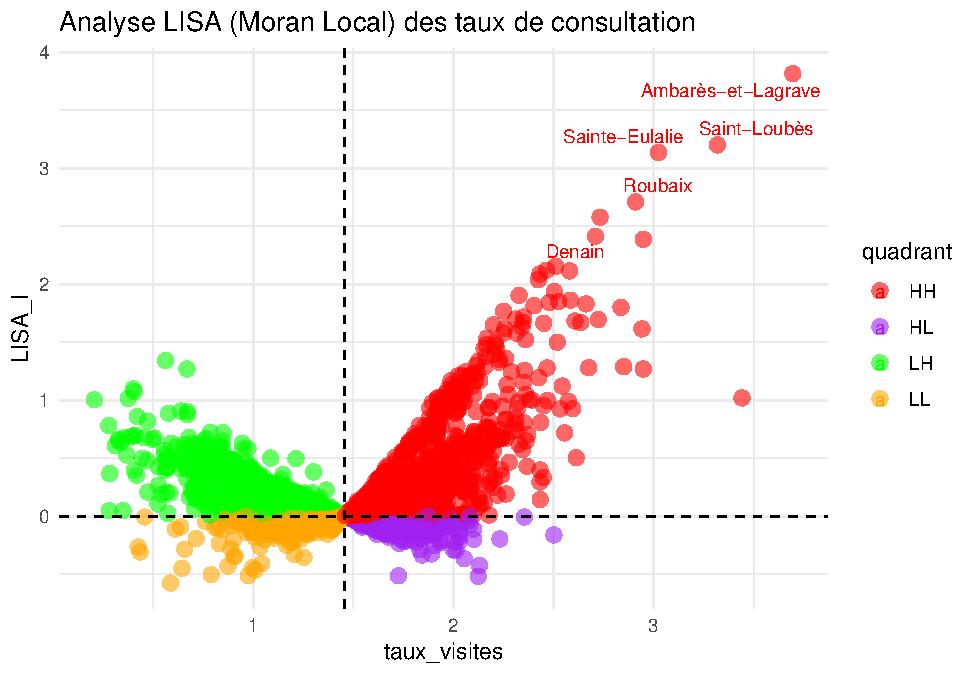
\includegraphics{4_Analyse_Descriptive_files/figure-latex/unnamed-chunk-20-1} 

}

\caption{Clusters sur la base du LISA}\label{fig:unnamed-chunk-20}
\end{figure}

\end{document}
